% Created 2021-07-13 mar 23:24
% Intended LaTeX compiler: pdflatex
\documentclass[11pt]{article}
\usepackage[utf8]{inputenc}
\usepackage[T1]{fontenc}
\usepackage{graphicx}
\usepackage{grffile}
\usepackage{longtable}
\usepackage{wrapfig}
\usepackage{rotating}
\usepackage[normalem]{ulem}
\usepackage{amsmath}
\usepackage{textcomp}
\usepackage{amssymb}
\usepackage{capt-of}
\usepackage{hyperref}
\author{Mundfaristoj, with help from the GPT-J}
\date{\today}
\title{Universe-416ZK}
\hypersetup{
 pdfauthor={Mundfaristoj, with help from the GPT-J},
 pdftitle={Universe-416ZK},
 pdfkeywords={},
 pdfsubject={},
 pdfcreator={Emacs 27.2 (Org mode 9.5)}, 
 pdflang={English}}
\begin{document}

\maketitle
\setcounter{tocdepth}{2}
\tableofcontents


\section*{\underline{Introduction}}
\label{sec:orgf38f8d2}
\subsection*{What is this ``worldbuilding'' thing you're talking about?}
\label{sec:orgbaf553c}
Acording to \href{https://www.fandomspot.com/worldbuilding/}{FandomSpot.com}, worldbuilding is
\begin{quote}
``the process of creating entire fantasy worlds from scratch, all while considering the logistics of these worlds to make them as believable as possible. Worldbuilding asks questions about the setting of a world, and then answers them, often in great detail.
Think of all the media you enjoy. Games. Movies. Television. Novels.
Most of them probably have a story.
If you get a bit more technical, those stories all take place somewhere. Literature teachers would call that the setting.
I think of that place as a “world” for each piece of creative work. So worldbuilding is really just the process of making those worlds.''
\end{quote}

\subsection*{Okay, what's your idea then?}
\label{sec:orgf623815}
Well\ldots{}
    Welcome to the Universe-419ZK World Building Project! This project is based on a fictional setting called the Universe-419ZK (not actually an abbreviation) which will eventually become a universe. It's designed to be a sandbox environment, where the creators can make up their own worlds as they go, without having to worry about ``canon'' at all! (\emph{we'll try to make it good}) This document/page is for posting the rules, laws, ideas, or anything else related to this universe. Feel free to post your suggestions in the \href{https://discord.gg/4UKUF78REF}{Discord Server}, but keep in mind, it'll be up to the project's creators to decide what gets added to the universe.

\emph{thanks to \href{https://bellard.org/textsynth/}{GPT-J} for giving us an introduction.}

\subsection*{Who are ``the creators''?}
\label{sec:org2a16939}
We're just some friends trying to worldbuild, we're slow at it though, so we could use some help!


\section*{\underline{Info}}
\label{sec:org2e7904c}
\subsection*{Species}
\label{sec:org3ab5808}
\subsubsection*{Aurun's Dogs}
\label{sec:org7b2e23d}
Aurun's Dogs or Aurunies for short.  They're similar to dogs in appearance but an intelligent species and can talk.  They're solitary and rarely group.  Aurun is the place where they were first discovered and that's where the majority of them reside.  The name of the species the Aurunies have for themselves is the Naaru, which is both plural and singular.
Aurunies are pretty serious and rarely speak.  When they do, whatever they say is going to be something pretty important.  Once in a few generations you get a jokester but they're far and few in that community.  Aurunies prefer to keep to themselves and thus have much disdain for other races.
Depending on which part of Aurun they inhabit, some are long haired and others are short haired.  Adult size is the same size as a border collie.

\begin{center}
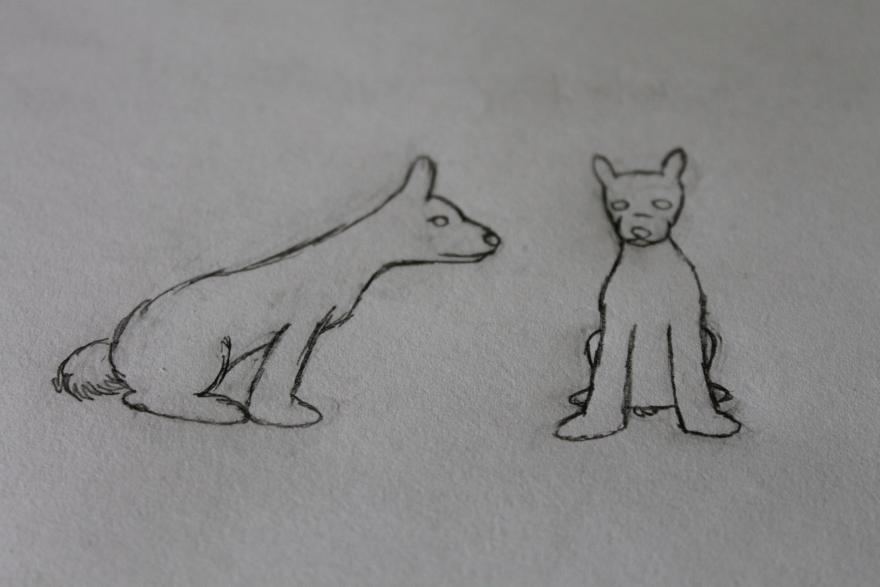
\includegraphics[width=.9\linewidth]{./assets/southern auruns dogs.jpg}
\end{center}\begin{center}
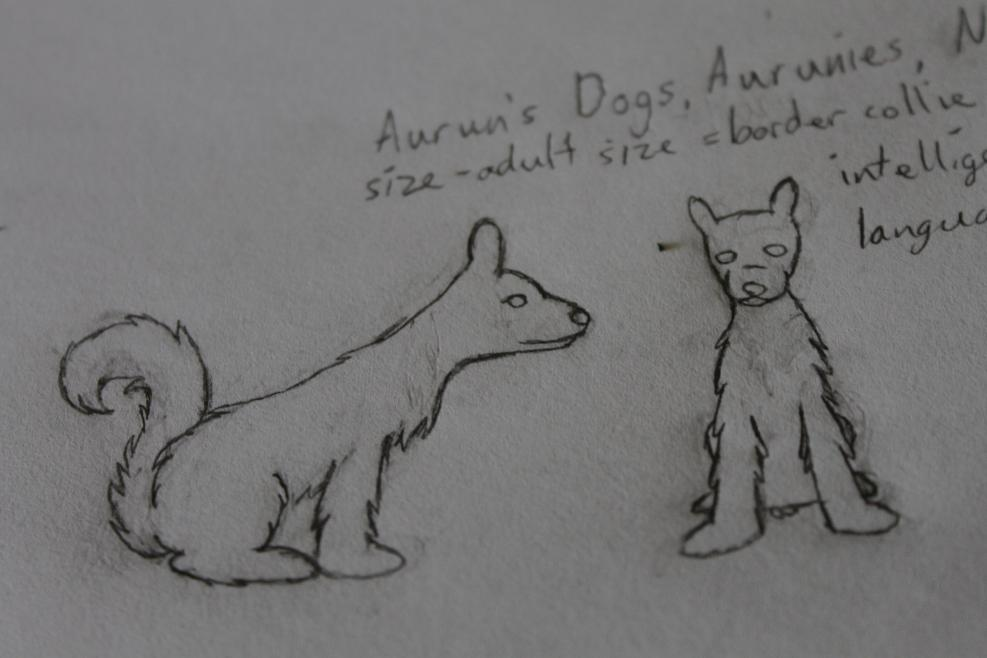
\includegraphics[width=.9\linewidth]{./assets/northern auruns dogs.JPG}
\end{center}
Southern and northern Aurun's dogs.
\subsubsection*{Rock men}
\label{sec:org175e613}
Structurally similar to humans, althought made out of rock.
They have incredible strength and can survive with no food nor water for extended periods of time, as well as having insane resistence. They can survive for up to 3 days without food.
They are vitually immune to the effect of ``Tired''.
If they die, they will fall back down into their original form and become a normal pile of rocks again.
They weigh around 400 pounds, stand 7 feet tall, and look like a brownish gray rock.
They're known to live for over 200 years, although the limit is unknown. A good example of this is the case of a rock man that lived 429 years.
Their digestive system makes them invulnerable to any known poison.
They are believed to have no emotions at all.
They live in small societies, and tend to have a society of men and one of women, regularly meeting.


\begin{itemize}
\item There are some variations of this species:
\label{sec:org6e5be6b}
\begin{itemize}
\item Lava men: They look like rock men, only bigger, taller, and can run faster than normal rock men.
\item Mountain rock men: Made from minerals and metals, they are slightly weaker than rock men, and can run on top of earth and stone for some distance, but aren't as strong. They are immune to fire, lava and can withstand temperatures way over 5000°C.
\end{itemize}
\end{itemize}

\subsubsection*{Gestalts:}
\label{sec:org87c1605}
Gestalts are usually shorter than the average human. Their bodies are very muscular and they tend to move with a loping gait. Many of them have a large, round head with enormous almond shaped eyes. Their skin is tinged with shades of red and sometimes blue.
The most common of which are the red/pink hair, but other gestalts have green, white and black hair among others.
Their bodies are formed from a special mineral, and so they can survive in air, water, and on dry land.
Their emotions are raw, intense and sometimes violent.
Gestalts are very tribal and have a great sense of loyalty to their people. They live in clans and tribes and they usually follow some sort of leader.
Gestalts are the hardest hitting race in the world, being able to defeat anything from the lightest creature to the strongest humans.
Gestalts hate humans, they have expressed in numerous ocasions that they want the world to be theirs.
Gestalts are known for being a very difficult race to kill, making them an even greater threat.

\begin{itemize}
\item Deformities
\label{sec:org556edd1}
Gestalts typically have one of two different types of common deformities:
\begin{itemize}
\item Head deformities:
One common head deformity is a single horn protruding from the front of their head. However, the horn can vary greatly. This can be any type of horn, from simple hair-like frills to large spikes that grow from the center of the head. These horns generally do not make the Gestalt look any less intimidating. In fact, it makes them appear larger, and more intimidating.

\item Face deformities:
The other common head deformity is a large round nose. The nose can vary from wide and large to small and narrow. Like head horns, the nose horns make the Gestalt look larger and more intimidating, but this time it is due to the nose's size. These noses can appear to be the same size as the horns, or much larger.
\end{itemize}
\end{itemize}

\subsection*{{\bfseries\sffamily TODO} Geography}
\label{sec:org63af123}
\subsection*{{\bfseries\sffamily TODO} Culture}
\label{sec:org3b13568}
\subsection*{Some Stories}
\label{sec:org557fc4c}
\subsubsection*{The Wandering Ghosts of Minstrade:}
\label{sec:orgde4d8cd}
\begin{quote}
Damn those specters.  Always floating about and wailing, ever so lost.  I despise going through Minstrade because of them.  Most of the time, ghosts only appear to their relatives but I've got the rather unfortunate ability to speak and interact with every ghost on this planet. Sometimes they're helpful and sometimes they're just a plain nuisance and they know it.  Recently, I had to deal with a lost Sijkh princess calling for her mummy.  Poor girl.  She got herself lost and like numerous before her, died before anyone could ever find her.  She was only around 7 years old.  For some reason, Minstrade seems to be the mecca for every ghost.

Every ghost just feels compelled to go there but nobody ever knows why.  Once they reach ghosthood, they eventually find their way to Minstrade, sight see, then return to where they came from or simply stay there.  There aren't any legends surrounding Minstrade, or at least none to explain why there's an abundance of ghosts there.  There are simply many ghost stories hanging around that place.
\end{quote}
\emph{Transcribed from the journal of explorer Isakov, date unknown}

\subsubsection*{Misterious recording}
\label{sec:org144e1e1}
\begin{quote}
\textbf{crackle}\ldots{} \textbf{static}\ldots{} \textbf{beep}
\textbf{thump\ldots{} thump\ldots{} thump\ldots{} CRASH}
\textbf{huff puff gasp}
``RUN! No Emily, DON'T look back! I'll be okay\ldots{} I PROMISE\ldots{} I WILL be waiting for you in the \textbf{bzzz} back home!''
``No, I \textbf{crzzzz} I can't leave without you by \textbf{bzz} I have to \textbf{bzz}''
\textbf{groaning\ldots{} creaking\ldots{} stomp}
``Don't worry, I will be fine, we made this shelter out of \textbf{zzzz} I'll hide, it can't see me, but THEY CAN DEFINITELY \textbf{crzzzz}
''I will be back for you\ldots{} I will come back with \textbf{bzzzz} to help you\ldots{} DON'T GIVE UP, WE'LL COME BACK!``
\textbf{whispers as the thumps get louder}
''I know you'll be back\ldots{} but I'm sorry, I should've told you from the start that I'm \textbf{beeeeeeeeeeep}``
\textbf{crackle}\ldots{} \textbf{static}
\end{quote}
\emph{from a mysterious sharp device emitting sound}

\subsection*{Some Trivia (We will probably expand on this later on)}
\label{sec:orgbd53c91}
\begin{itemize}
\item There are some places where inteligent species haven't gone yet because of dangers.
\item Scientists at some point figured out how to change the gender of a fetus using vegetable extract.
\end{itemize}
\end{document}
